% !TeX root = ../sustechthesis-example.tex

\chapter[基于FPGA的RTMQ测控系统]{基于FPGA的RTMQ测控系统}

% \textcolor{red}{
% 这部分参考RTMQ的相关专利和文档介绍整个测控系统的情况... 
% }

量子物理实验系统常常涉及到一些物理量的精确调控和测量,这既包括量上的精确性,也包括时间上的精确性。因此量子物理实验系统对测量和控制性能提出了很多新的要求,其中十分关键的一点就是对测控系统实时性的要求。

目前实时系统在医疗、加工、汽车等行业都有较多的应用,实时系统具有响应快、延迟短等特点,其响应延迟和计时精度通常在毫秒至微秒量级,这一精度已经能满足当前诸多传统行业的控制需求。现有的实时系统一般使用主频在数百MHz至GHz量级的通用微处理器或微控制器作为控制的主体,以计时器中断和时间片分配等方式实现实时控制。这一方案成立的前提在于,所需的时间控制精度与指令执行频率之间有3-6个数量级的差异,因而通用处理器架构中存在的一些诸如分支预判、乱序执行等导致指令执行顺序不确定的因素以及中断系统中存在的现场保护、控制权交接等额外开销导致的时间控制不确定性可以忽略不计。

然而近来随着量子技术的发展,量子物理实验系统也开始产生对数据处理、复杂流程控制和实时控制的需求。不同于传统行业,量子物理实验系统对时间控制的精度和分辨率的要求在纳秒量级、延迟要求在百纳秒至数十微秒量级,与当前微处理器的主频相当,从而前述的现有的实时控制方案难以满足需求。

因此早年在量子物理实验领域内,通常用FPGA(现场可编程门阵列)设计特定的时序脉冲发生器来产生高时间精度的脉冲序列,以此作为其它实验设备的触发信号,进行准确的时序控制。然而,这种方案的灵活性较差,只能产生预定的序列,无法在实验中对实验数据进行即时的处理,或根据实验的中间结果对后续的流程进行及时的调整。近年来随着量子算法的发展,实验方案越来越复杂,实验流程中开始包含快速反馈的结构,即在实验过程中对实验目标进行测量,获得一些中间结果,而后对中间结果进行计算和处理,并进而确定后续的实验流程。中间结果的处理和后续流程的确定,一般要求在数十纳秒至数十微秒量级的时间内完成,并且执行时刻必须要严格确定。这要求实验的测控系统具有通用计算的能力,简单的时序脉冲发生器无法满足这一要求。

当前领域内针对此问题的主要解决思路为,另置一与时序脉冲发生器紧密连接的通用微处理器,用来对实验数据进行即时处理和产生时序脉冲发生器的后续输出时序。这一方案能较好的满足系统规模较小且实验时序不太复杂的情形下的实时控制需求。然而,这一方案的问题之一在于,微处理器和时序脉冲发生器依然是相互独立的两个个体,而微处理器的执行时序有其内在不确定性;二者之间要保持同步,或者需要频繁地相互交换触发信号,或者需要在时序设计上预留出充足的余量以覆盖此不确定性的最坏情形,总之都会复杂化时序的设计并产生时间浪费。

这一方案的另一问题在于,当系统规模较大,一个时序脉冲发生器无法控制整个系统时,就需要同时使用多个时序脉冲发生器,而一个微处理器同时处理过多的实验数据、同时控制过多的时序脉冲发生器,将不可避免的产生拥塞,这会进一步加剧前述的同步性问题。而如果同时使用多个微处理器,则不同微处理器之间的同步性又将成为问题;当前主流的微处理器架构和指令集都是针对通用计算而优化的,主流的微处理器使用的通信协议都是针对高吞吐率而优化的,二者都难以实现精确的时序同步。

\section[RTMQ实时系统架构介绍]{RTMQ实时系统架构介绍}

对于离子阱量子计算研究来说,一种实时性更强、拓展性更好、更灵活的测控系统十分重要。我们实验中对系统的控制和测量采用一种叫RTMQ的系统架构来实现。RTMQ系统架构提供了一种新的量子物理实验平台实时测控系统架构,解决了上述的不足。在RTMQ系统架构中,通用计算和时序控制由同一微处理器实现,因此避免了两个独立的模块之间同步性的问题;同时树状结构的系统中每个节点都具有通用计算的能力,因此可以实现计算任务的分布式处理,避免了拥塞的问题。

\begin{figure}
    \centering
    \caption[RTMQ系统架构示意图]{RTMQ系统架构示意图\label{fig:rtmq_nodes_and_leaves_structure}}
    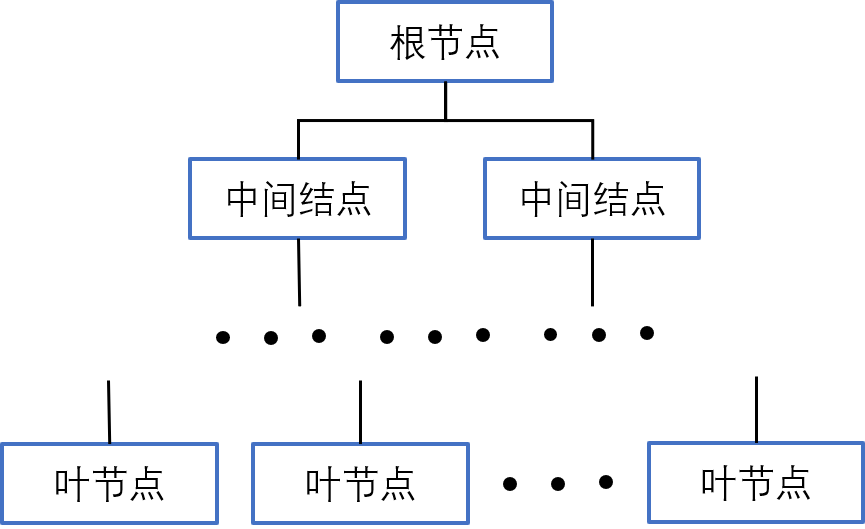
\includegraphics[width=0.6\linewidth]{rtmq/rtmq_nodes_and_leaves_structure}
\end{figure}

RTMQ(用于量子物理实验的实时微系统,RealTime Microsystem for Quantum physics)架构主要用于基于FPGA或ASIC的兼具通用计算和高精度时序控制能力的微系统。系统的整体结构为树状结构,如图\ref{fig:rtmq_nodes_and_leaves_structure}所示,系统包含一个根节点,多个中间结点和多个叶节点;根节点通过网络、USB等方式与控制计算机相连。不同节点可位于同一PCB上,亦可位于不同PCB上。

\begin{figure}
    \centering
    \caption[RTMQ系统架构节点示意图]{RTMQ系统架构节点示意图\label{fig:rtmq_board_overal_structure}}
    
\includegraphics[width=0.4\linewidth]{rtmq/rtmq_board_overal_structure}
\end{figure}

一般而言一个板卡具有如图\ref{fig:rtmq_board_overal_structure}所示的结构,板卡上的FPGA或ASIC包含一个RTMQ节点,RTMQ节点通过控制FPGA或ASIC的输入输出与数模/模数转换等各类功能芯片进行交互以实现所需功能,同时通过实时通信链路与其上级和下级节点连接。

\begin{figure}
    \centering
    \caption[RTMQ系统架构节点内部模块示意图]{RTMQ系统架构节点内部模块示意图\label{fig:rtmq_board_inner_structure}}
    
\includegraphics[width=1.0\linewidth]{rtmq/rtmq_board_inner_structure}
\end{figure}

一个RTMQ节点的内部模块儿如图\ref{fig:rtmq_board_inner_structure}所示,包含一个32位的微处理器、一个寄存器文件、一系列外设模块和一个链路管理模块。其中微处理器包含流控制器、计时器、异常管理模块、触发管理模块和算术逻辑单元5个子模块;寄存器文件包含多个寄存器;外设可分为系统外设和功能外设,系统外设包括指令缓存、数据缓存、节点信息只读存储器以及地址栈和数据栈,功能外设用于实现具体的逻辑或时序功能,可包含多个。

RTMQ架构中包含的微处理器可受指令控制进入挂起状态,而挂起状态可受计时器或触发管理模块的控制恢复正常运行,如此,微处理器的指令流便可以按一定的时间间隔对齐或与外部信号对齐。同时,节点中的系统外设和功能外设的行为受关联寄存器的读写控制,即微处理器的指令与系统各模块的功能和时序有严格的对应关系。因此,本发明提供的架构可实现实时控制与通用计算在指令流层面的结合。
而配置指令插入中断的机制确保了节点对其下级节点的绝对控制,即使下级节点的微处理器处于挂起状态,依然不受影响。配置指令插入中断配合具有确定通信延迟的实时通信链路系统,即可实现时序确定的跨节点的即时反馈控制。

此外,RTMQ架构中每个节点都具有通用计算和时序控制能力,如此,大多数通用计算和时序生成都可以在叶节点或较近的中间结点完成,对于大规模系统不存在拥塞的问题,具有良好的可扩展性。


\section[测控硬件组成]{测控硬件组成}
\textcolor{red}{
1. 展示实物板卡照片;}

\textcolor{red}{
2. 结合照片给出主要器件清单及其介绍(参考专利:一种量子物理实验平台的实时测控系统架构);}
\section[软件API]{软件API}
\textcolor{red}{
1. 介绍软件API的功能和使用(可选,根据情况看吧,怎么介绍还没想好);}


\section[基于FPGA的数字超前进位加法器]{基于FPGA的数字超前进位加法器}
\textcolor{red}{
1. 介绍数字加法器功能、逻辑图、Vivado中的实现、局限性;}

\textcolor{red}{
2. 介绍超前进位加法器的优势、逻辑图、Vivado中的实现;}

\section[基于FPGA的数字Booth乘法器]{基于FPGA的数字Booth乘法器}
\textcolor{red}{
1. 介绍数字Booth乘法器功能、逻辑图、Vivado中的实现、优势;}

\section[基于FPGA的数字PID]{基于FPGA的数字PID}
\textcolor{red}{
1. 介绍数字PID功能、逻辑图、Vivado中的实现、优势;}

\section[基于FPGA的通用数字滤波器]{基于FPGA的通用数字滤波器}
\textcolor{red}{
1. 介绍数字滤波器功能、种类、基本原理,比如有限冲激响应滤波器、无限冲激响应滤波器等等;}

\textcolor{red}{
2. 介绍数字通用滤波器功能、逻辑图、Vivado中的实现、优势;}




